\section{Security Analysis}
\label{sec:security}

Every result in this section is \emph{proxy-evaluated under a specific, named attacker}. No formal, cryptographic, semantic, or differential-privacy claim is made. The phrase ``is bounded under tested proxy attackers'' replaces ``is secure'' throughout. The mapping between proxy attackers and claim status is summarized in \Cref{tab:security-proxy-summary} and \Cref{fig:security-risk-matrix}, and pinned in the claims-mapping appendix (\Cref{app:claims}).

\paragraph{Risk-level taxonomy.}
We adopt the four-level taxonomy produced by the artifact pipeline: \texttt{low}---under the named attacker, the recovered signal is close to random chance; \texttt{medium}---a residual signal exists but is not strong enough to recover the target; \texttt{needs\_more\_evaluation}---the attackers we ran do not succeed, but a stronger attacker may; \texttt{high}---the attacker succeeds, this is reported as a known leakage channel.

\subsection{Transcript obfuscation}
\label{sec:security:transcript}
Under the full mitigation bundle (fresh per-call permutation $+$ dense Linear sandwich $+$ boundary pad), the GPU-visible transcript per call is $(\Xt, \Wt, \At, \Bt, \Kt, \Vt, \Yt)$. We instantiate four adaptive proxy attackers on this transcript:

\begin{itemize}[leftmargin=*, nosep]
  \item \textbf{Ridge inverter} on $(\Xt, \Yt)$ pairs. \emph{Bounded near random chance in our evaluated setting.}
  \item \textbf{Small MLP inverter}. \emph{Bounded near random chance in our evaluated setting.}
  \item \textbf{Signature- and Sinkhorn-based permutation recovery} against permutation islands. \emph{Bounded near random chance under fresh per-call masks; this is proxy-evaluated, not formally proven.}
  \item \textbf{Membership-style linkability AUC} on two masked traces of the same plain input. \emph{Bounded near $0.5$ in our tested configurations.}
\end{itemize}
Status: \texttt{proxy\_supported}.

\subsection{Activation recovery and linkability}
\label{sec:security:activation}
For the modern-decoder block and model wrappers, the same attacker family is evaluated against block-level masked activations and model-level real-token traces. Under the full mitigation bundle, the worst-case attacker accuracy stays near random chance in our tests; the artifact tags this as \texttt{needs\_more\_evaluation}, since we cannot exclude a stronger attacker. The safe wording is: \emph{under our adaptive proxy attackers, the full mitigation bundle keeps the worst-case attacker close to random chance in our tested configurations.}

\subsection{KV cache and generation trace}
\label{sec:security:kv}
The KV cache invariant (\Cref{thm:attention}) preserves attention scores; the masked cache is randomized per call by $\NK, \NV$. A dedicated \emph{generation-trace} recovery attacker---one that takes the full masked decode transcript and attempts to recover the prompt-to-output mapping in plain space---is not evaluated in this paper and is therefore reported as \texttt{needs\_more\_evaluation}. The output tokens themselves are visible to the GPU by the threat model (\Cref{sec:threat}); this is an allowed leakage channel.

\subsection{LoRA adapter extraction}
\label{sec:security:adapter}
The adapter extraction attacker observes $(\Xt, \At, \Bt, \Yt)$ over multiple calls and attempts to recover $(\A, \B)$ (or any rotated version thereof). Under fresh masks per call $+$ rank padding, the attacker's recovery is bounded; the membership-style linkability AUC is reduced by $\Delta\text{AUC} = +0.463$ versus the \texttt{fixed\_masks\_fixed\_u} baseline. Status: \texttt{proxy\_supported}, risk \texttt{needs\_more\_evaluation}.

\subsection{Gradient leakage}
\label{sec:security:gradient}
The gradient extraction attacker observes $(\Gt, \widetilde{\partial\A}, \widetilde{\partial\B})$ over multiple calls~\cite{zhu2019dlg, zhao2020idlg}. Under fresh masks $+$ pad, the gradient-side membership linkability AUC is reduced by $\Delta\text{AUC} = +0.478$ versus the \texttt{fixed\_masks\_fixed\_u} baseline. Status: \texttt{proxy\_supported}, risk \texttt{needs\_more\_evaluation}.

\subsection{Rank leakage and dummy hardening}
\label{sec:security:rank}
Rank padding (\Cref{sec:design:rank-pad}) hides the true rank $\rtrue$ from tensor shape; $\rpad$ itself remains visible. We evaluate four spectral-inference proxy detectors (spectral cliff, energy, elbow, ensemble). Across $\rtrue \in \{2, 4, 8\}$ with \texttt{paired\_cancellation\_dummy}, the worst-case spectral-inference risk is \texttt{needs\_more\_evaluation} and the gradient-inference risk is \texttt{high}. With the Stage 7.4 stronger-dummy ensemble: spectral-rank-inference worst-case \texttt{high}; gradient-rank-inference worst-case \texttt{high}; dummy-strategy classifier $0.476$ vs chance $0.143$ (risk \texttt{medium}); cross-layer linkage \texttt{low}.

We faithfully report all four risk levels, including the high ones. Specifically, \textbf{we do not claim that rank padding hides the LoRA rank cryptographically, and we do not claim $\rpad$ is hidden}.

\subsection{Timing and metadata}
\label{sec:security:timing}
A cost-model timing classifier on training-step latency reaches above-random accuracy with constant-time mode off. With the \texttt{proxy\_equalized} mode on, the worst-case classifier accuracy drops to $0.5124$ (near chance for a two-class task). Risk level: \texttt{low}. This is a cost-model proxy only; we do not claim real wall-time hardness and we do not evaluate hardware side-channels~\cite{kocher2019spectre, vanbulck2018foreshadow}.

\subsection{Cross-layer linkage}
\label{sec:security:crosslayer}
Cross-layer adapter linkage is \texttt{high} under shared-mask/shared-$\UU$ baselines (by construction; the baseline does not refresh masks). Under fresh masks per module $+$ paired cancellation, the cross-layer linkability AUC stays near $0.5$ across the tested multi-layer configuration. The Stage 7.4 stronger-dummy ensemble preserves cross-layer linkage at \texttt{low}.

\subsection{Claims boundary}
\label{sec:security:boundary}
\Cref{fig:security-risk-matrix} summarizes risk levels across the $14$ proxy-attacker rows in \Cref{tab:security-proxy-summary}. To be explicit, we do \emph{not} claim that the system is secure; we do \emph{not} claim semantic, cryptographic, or formal indistinguishability; we do \emph{not} claim resistance to a compromised TEE; we do \emph{not} claim resistance to hardware side-channels; we do \emph{not} claim the padded LoRA rank is hidden; we do \emph{not} claim real TEE wall-time. We \emph{do} claim, under the named proxy attackers on the tested configurations, that the worst-case proxy classifier is reduced to near random chance for the items the artifact labels \texttt{low}; residual leakage in \texttt{needs\_more\_evaluation}, \texttt{medium}, and \texttt{high} items is reported faithfully and not re-classified.

\begin{figure}[h]
\centering
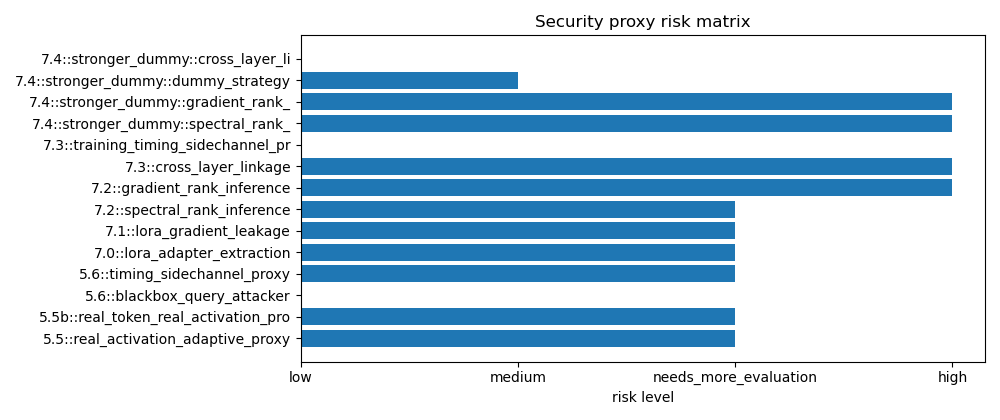
\includegraphics[width=0.92\linewidth]{figures/security_risk_matrix.png}
\caption{Security risk matrix across the $14$ proxy-attacker rows of \Cref{tab:security-proxy-summary}. \texttt{low} cells are bounded close to random chance in our tests under the named attacker; \texttt{needs\_more\_evaluation} cells are open under stronger attackers; \texttt{medium} and \texttt{high} cells are reported as residual leakage. Every row is proxy-supported only.}
\label{fig:security-risk-matrix}
\end{figure}

% Auto-generated by paper_artifact_consolidation
\begin{table}[h]
\centering
\small
\caption{Security Proxy Summary}
\label{tab:security\_proxy\_summary}
\begin{tabular}{llllllllll}
\toprule
stage & attack\_family & target & strategy & metric & value & risk\_level & recommendation & artifact\_path & claim\_supported \\
\midrule
5.5 & real\_activation\_adaptive\_proxy & modern\_decoder\_block & ridge\_linear\_plus\_mlp & linkability\_auc & None & needs\_more\_evaluation & fresh\_perm + sandwich + pad & outputs/real\_activation\_attacks.json & proxy-supported only \\
5.5b & real\_token\_real\_activation\_proxy & modern\_decoder\_model\_level & real\_token\_proxy & linkability\_auc & None & needs\_more\_evaluation & fresh\_perm + sandwich + pad & outputs/real\_token\_activation\_attacks.json & proxy-supported only \\
5.6 & blackbox\_query\_attacker & modern\_decoder\_model\_level & n/a & best\_distinguishability & None & low & exact-token-match guarantee & outputs/stronger\_attackers.json & proxy-supported only \\
5.6 & timing\_sidechannel\_proxy & modern\_decoder\_model\_level & off & best\_classification\_accuracy & None & None & constant\_time\_decode\_mode=proxy\_equalized & outputs/stronger\_attackers.json & proxy-supported only (cost-model) \\
7.0 & lora\_adapter\_extraction & synthetic\_lora\_linear & fresh\_masks\_fresh\_u\_with\_pad & linkability\_auc\_summary & fresh masks reduce membership-style linkability (Δ AUC = +0.463 vs fixed\_mask... & needs\_more\_evaluation & fresh masks + pad & outputs/lora\_security\_proxy.json & proxy-supported only \\
7.1 & lora\_gradient\_leakage & synthetic\_lora\_linear\_backward & fresh\_masks\_fresh\_u\_with\_pad & linkability\_summary & fresh masks reduce gradient-side membership linkability (Δ AUC = +0.478 vs fi... & needs\_more\_evaluation & fresh masks + pad; rank still visible from shape & outputs/lora\_gradient\_security\_proxy.json & proxy-supported only \\
7.2 & spectral\_rank\_inference & rank\_padded\_lora & paired\_cancellation\_dummy & spectral\_inference\_summary & Across true\_ranks=[2, 4, 8] with dummy\_strategy='paired\_cancellation\_dummy', ... & needs\_more\_evaluation & use stronger dummy distributions (Stage 7.4) & outputs/lora\_rank\_security\_proxy.json & proxy-supported only \\
7.2 & gradient\_rank\_inference & rank\_padded\_lora & paired\_cancellation\_dummy & gradient\_inference\_summary & Gradient-side spectral inference risk under the same dummy strategy is **high**. & high & use stronger dummy distributions (Stage 7.4) & outputs/lora\_rank\_security\_proxy.json & proxy-supported only \\
7.3 & cross\_layer\_linkage & multi\_layer\_rank\_padded\_lora & fresh\_masks\_independent\_u & cross\_layer\_linkage\_summary & Cross-layer linkage risk under multi-layer strategies is **high** (worst-case). & high & fresh masks per module + paired cancellation & outputs/multilayer\_lora\_security\_proxy.json & proxy-supported only \\
7.3 & training\_timing\_sidechannel\_proxy & lora\_training\_step\_cost\_model & proxy\_equalized & max\_classification\_accuracy\_proxy\_equalized & 0.5123697916666666 & low & proxy\_equalized constant-time mode & outputs/lora\_training\_timing\_proxy.json & proxy-supported only (cost-model) \\
7.4 & stronger\_dummy::spectral\_rank\_inference & rank\_padded\_lora\_with\_stronger\_dummies & ensemble & spectral\_summary & Worst spectral rank inference risk across strategies: **high**. & high & spectrum\_matched\_dummy / mixed\_dummy\_ensemble & outputs/lora\_stronger\_dummy\_security\_proxy.json & proxy-supported only \\
7.4 & stronger\_dummy::gradient\_rank\_inference & rank\_padded\_lora\_with\_stronger\_dummies & ensemble & gradient\_summary & Worst gradient rank inference risk across strategies: **high**. & high & spectrum\_matched\_dummy / mixed\_dummy\_ensemble & outputs/lora\_stronger\_dummy\_security\_proxy.json & proxy-supported only \\
7.4 & stronger\_dummy::dummy\_strategy\_classification & rank\_padded\_lora\_with\_stronger\_dummies & ensemble & dummy\_strategy\_classification\_summary & Dummy strategy classifier accuracy: 0.476 (chance 0.143), risk **medium**. & medium & spectrum\_matched\_dummy / mixed\_dummy\_ensemble & outputs/lora\_stronger\_dummy\_security\_proxy.json & proxy-supported only \\
7.4 & stronger\_dummy::cross\_layer\_linkage & rank\_padded\_lora\_with\_stronger\_dummies & ensemble & cross\_layer\_linkage\_summary & Worst cross-layer linkage risk across strategies: **low**. & low & spectrum\_matched\_dummy / mixed\_dummy\_ensemble & outputs/lora\_stronger\_dummy\_security\_proxy.json & proxy-supported only \\
\bottomrule
\end{tabular}
\end{table}

